% Created by tikzDevice version 0.12.3.1 on 2021-12-04 14:31:34
% !TEX encoding = UTF-8 Unicode
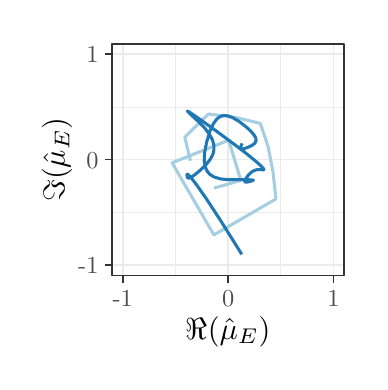
\begin{tikzpicture}[x=1pt,y=1pt]
\definecolor{fillColor}{RGB}{255,255,255}
\begin{scope}
\definecolor{drawColor}{RGB}{255,255,255}
\definecolor{fillColor}{RGB}{255,255,255}

\path[draw=drawColor,line width= 0.6pt,line join=round,line cap=round,fill=fillColor] (  0.22,  0.00) rectangle (119.75,119.97);
\end{scope}
\begin{scope}
\definecolor{fillColor}{RGB}{255,255,255}

\path[fill=fillColor] ( 30.47, 30.69) rectangle (114.25,114.47);
\definecolor{drawColor}{gray}{0.92}

\path[draw=drawColor,line width= 0.3pt,line join=round] ( 30.47, 53.54) --
	(114.25, 53.54);

\path[draw=drawColor,line width= 0.3pt,line join=round] ( 30.47, 91.62) --
	(114.25, 91.62);

\path[draw=drawColor,line width= 0.3pt,line join=round] ( 53.32, 30.69) --
	( 53.32,114.47);

\path[draw=drawColor,line width= 0.3pt,line join=round] ( 91.40, 30.69) --
	( 91.40,114.47);

\path[draw=drawColor,line width= 0.6pt,line join=round] ( 30.47, 34.49) --
	(114.25, 34.49);

\path[draw=drawColor,line width= 0.6pt,line join=round] ( 30.47, 72.58) --
	(114.25, 72.58);

\path[draw=drawColor,line width= 0.6pt,line join=round] ( 30.47,110.66) --
	(114.25,110.66);

\path[draw=drawColor,line width= 0.6pt,line join=round] ( 34.27, 30.69) --
	( 34.27,114.47);

\path[draw=drawColor,line width= 0.6pt,line join=round] ( 72.36, 30.69) --
	( 72.36,114.47);

\path[draw=drawColor,line width= 0.6pt,line join=round] (110.44, 30.69) --
	(110.44,114.47);
\definecolor{drawColor}{RGB}{166,206,227}

\path[draw=drawColor,line width= 1.1pt,line join=round] ( 67.23, 62.30) --
	( 76.96, 65.06) --
	( 72.56, 79.60) --
	( 52.10, 71.44) --
	( 67.21, 45.38) --
	( 89.63, 58.37) --
	( 88.56, 68.29) --
	( 86.72, 77.57) --
	( 83.97, 85.68) --
	( 75.05, 87.84) --
	( 65.24, 89.08) --
	( 56.68, 80.71) --
	( 58.72, 72.18);
\definecolor{drawColor}{RGB}{31,120,180}

\path[draw=drawColor,line width= 1.1pt,line join=round] ( 77.40, 78.46) --
	( 77.02, 77.53) --
	( 76.88, 76.96) --
	( 76.89, 76.65) --
	( 76.99, 76.49) --
	( 77.20, 76.41) --
	( 77.62, 76.43) --
	( 78.36, 76.61) --
	( 79.55, 77.05) --
	( 80.99, 77.75) --
	( 81.88, 78.41) --
	( 82.32, 79.03) --
	( 82.46, 79.66) --
	( 82.32, 80.40) --
	( 81.81, 81.38) --
	( 80.74, 82.67) --
	( 78.93, 84.37) --
	( 76.25, 86.43) --
	( 73.87, 87.82) --
	( 72.04, 88.44) --
	( 70.60, 88.50) --
	( 69.38, 88.11) --
	( 68.22, 87.21) --
	( 67.05, 85.61) --
	( 65.84, 83.04) --
	( 64.65, 79.18) --
	( 63.86, 75.17) --
	( 63.72, 72.19) --
	( 64.05, 70.01) --
	( 64.76, 68.41) --
	( 65.83, 67.20) --
	( 67.37, 66.27) --
	( 69.59, 65.62) --
	( 72.71, 65.32) --
	( 76.39, 65.35) --
	( 78.92, 65.35) --
	( 80.42, 65.29) --
	( 81.16, 65.22) --
	( 81.42, 65.17) --
	( 81.45, 65.13) --
	( 81.36, 65.07) --
	( 80.94, 64.91) --
	( 80.00, 64.64) --
	( 79.21, 64.49) --
	( 78.74, 64.47) --
	( 78.50, 64.52) --
	( 78.39, 64.61) --
	( 78.35, 64.76) --
	( 78.41, 65.03) --
	( 78.63, 65.50) --
	( 79.10, 66.24) --
	( 79.72, 67.04) --
	( 80.34, 67.68) --
	( 80.95, 68.17) --
	( 81.57, 68.54) --
	( 82.20, 68.80) --
	( 82.87, 68.95) --
	( 83.58, 69.01) --
	( 84.35, 68.97) --
	( 85.04, 68.89) --
	( 85.26, 68.94) --
	( 85.27, 69.07) --
	( 85.01, 69.48) --
	( 84.14, 70.40) --
	( 82.31, 72.04) --
	( 79.15, 74.62) --
	( 74.27, 78.35) --
	( 67.61, 83.26) --
	( 62.49, 86.93) --
	( 59.52, 88.99) --
	( 58.11, 89.90) --
	( 57.67, 90.14) --
	( 57.64, 90.13) --
	( 57.87, 89.85) --
	( 58.86, 88.87) --
	( 61.21, 86.70) --
	( 63.90, 83.99) --
	( 65.68, 81.65) --
	( 66.73, 79.61) --
	( 67.22, 77.79) --
	( 67.23, 76.08) --
	( 66.80, 74.38) --
	( 65.83, 72.58) --
	( 64.21, 70.59) --
	( 62.09, 68.60) --
	( 60.46, 67.24) --
	( 59.32, 66.44) --
	( 58.57, 66.04) --
	( 58.11, 65.92) --
	( 57.83, 65.96) --
	( 57.65, 66.13) --
	( 57.52, 66.50) --
	( 57.48, 67.13) --
	( 57.57, 67.33) --
	( 57.88, 67.18) --
	( 58.83, 66.22) --
	( 60.84, 63.65) --
	( 64.32, 58.69) --
	( 69.66, 50.54) --
	( 77.27, 38.39);
\definecolor{drawColor}{gray}{0.20}

\path[draw=drawColor,line width= 0.6pt,line join=round,line cap=round] ( 30.47, 30.69) rectangle (114.25,114.47);
\end{scope}
\begin{scope}
\definecolor{drawColor}{gray}{0.30}

\node[text=drawColor,anchor=base east,inner sep=0pt, outer sep=0pt, scale=  0.88] at ( 25.52, 31.46) {-1};

\node[text=drawColor,anchor=base east,inner sep=0pt, outer sep=0pt, scale=  0.88] at ( 25.52, 69.55) {0};

\node[text=drawColor,anchor=base east,inner sep=0pt, outer sep=0pt, scale=  0.88] at ( 25.52,107.63) {1};
\end{scope}
\begin{scope}
\definecolor{drawColor}{gray}{0.20}

\path[draw=drawColor,line width= 0.6pt,line join=round] ( 27.72, 34.49) --
	( 30.47, 34.49);

\path[draw=drawColor,line width= 0.6pt,line join=round] ( 27.72, 72.58) --
	( 30.47, 72.58);

\path[draw=drawColor,line width= 0.6pt,line join=round] ( 27.72,110.66) --
	( 30.47,110.66);
\end{scope}
\begin{scope}
\definecolor{drawColor}{gray}{0.20}

\path[draw=drawColor,line width= 0.6pt,line join=round] ( 34.27, 27.94) --
	( 34.27, 30.69);

\path[draw=drawColor,line width= 0.6pt,line join=round] ( 72.36, 27.94) --
	( 72.36, 30.69);

\path[draw=drawColor,line width= 0.6pt,line join=round] (110.44, 27.94) --
	(110.44, 30.69);
\end{scope}
\begin{scope}
\definecolor{drawColor}{gray}{0.30}

\node[text=drawColor,anchor=base,inner sep=0pt, outer sep=0pt, scale=  0.88] at ( 34.27, 19.68) {-1};

\node[text=drawColor,anchor=base,inner sep=0pt, outer sep=0pt, scale=  0.88] at ( 72.36, 19.68) {0};

\node[text=drawColor,anchor=base,inner sep=0pt, outer sep=0pt, scale=  0.88] at (110.44, 19.68) {1};
\end{scope}
\begin{scope}
\definecolor{drawColor}{RGB}{0,0,0}

\node[text=drawColor,anchor=base,inner sep=0pt, outer sep=0pt, scale=  1.10] at ( 72.36,  7.64) {$\Re(\hat\mu_E)$};
\end{scope}
\begin{scope}
\definecolor{drawColor}{RGB}{0,0,0}

\node[text=drawColor,rotate= 90.00,anchor=base,inner sep=0pt, outer sep=0pt, scale=  1.10] at ( 13.30, 72.58) {$\Im(\hat\mu_E)$};
\end{scope}
\end{tikzpicture}
